\documentclass[a4paper,11pt]{report}
\usepackage[french]{babel}
\usepackage[T1]{fontenc}
\usepackage[utf8]{inputenc}
\usepackage{lmodern}
\usepackage{microtype}
\usepackage{hyperref}
\usepackage{tabulary}
\usepackage{framed}
\usepackage{fancyhdr}
\usepackage{amsmath}
\usepackage{bbm}
\usepackage{graphicx}

\newcommand{\latin}[1]{\textit{#1}}

\pagestyle{empty}

\pagestyle{fancy}
\fancyhead{}
\renewcommand{\headrulewidth}{0.5pt}
\fancyhead[R]{\textit{\nouppercase{\rightmark}}}
\fancyfoot{}
\renewcommand{\footrulewidth}{0.5pt}
\fancyfoot[L]{\textit{\nouppercase{\leftmark}}}
\fancyfoot[R]{\thepage}

\begin{document}
	\begin{titlepage}
		\vspace*{\stretch{2}}
		\begin{center}
			\large\bfseries\itshape Projet SPECIF\\
		\end{center}
		\noindent\rule{\linewidth}{3pt}

		\begin{center}
			\Huge\bfseries\itshape RAPPORT\\
		\end{center}
		
		\noindent\rule{\linewidth}{3pt}
		\begin{center}
			\bfseries
			\large Processeur
			
		\end{center}
		\vspace*{\stretch{2}}
		\begin{center}
			Réalisé par \bfseries \itshape DOAN Cao Sang
		\end{center}
		\begin{center}
			16 Avril 2015
		\end{center}
	\end{titlepage}

\chapter{CPU}
	\begin{framed}
		\begin{verbatim}
		node cpu(gen: bool^2; in: bool^2) returns (out: bool^4);

		--gen: 1er bit désigne type de requête, 2eme bit désigne 
			l'adresse de données
		--in: désigne 2 informations data ou ack, ces informations 
			sont validées si 2eme bit vaut 1

		--out: typedata, adresse data, data, valid

		var ok: bool;

		let
		out[0] = if ok then true -> gen[0] else false;
		out[1] = if ok then true -> gen[1] else false;
		out[2] = if ok and out[0] then not out[1]
                else if ok and out[1] then pre out[2]
                    else false;
		out[3] = if ok then true else false;

		ok = true -> if pre in[1] then true
             else false
			;
		tel;
	\end{verbatim}
	\end{framed}
	
	Le CPU qui génère les requête selon la demande de l'utilisateur à travers l'entrée $gen$ de 2 bits, le $1^{er}$ bit définit le type de requête, le $2^{ème}$ bit definit l'adresse de données demandée. Tant que l'a première requête n'a pas eu la réponse du cache, le processeur se bloque jusqu'à quand il reçoit la réponse valide du cache. Dès que il reçoit la réponse valide, il génère automatiquement la nouvelle requête.
	
	\begin{figure}[!htbp]
		\centering
		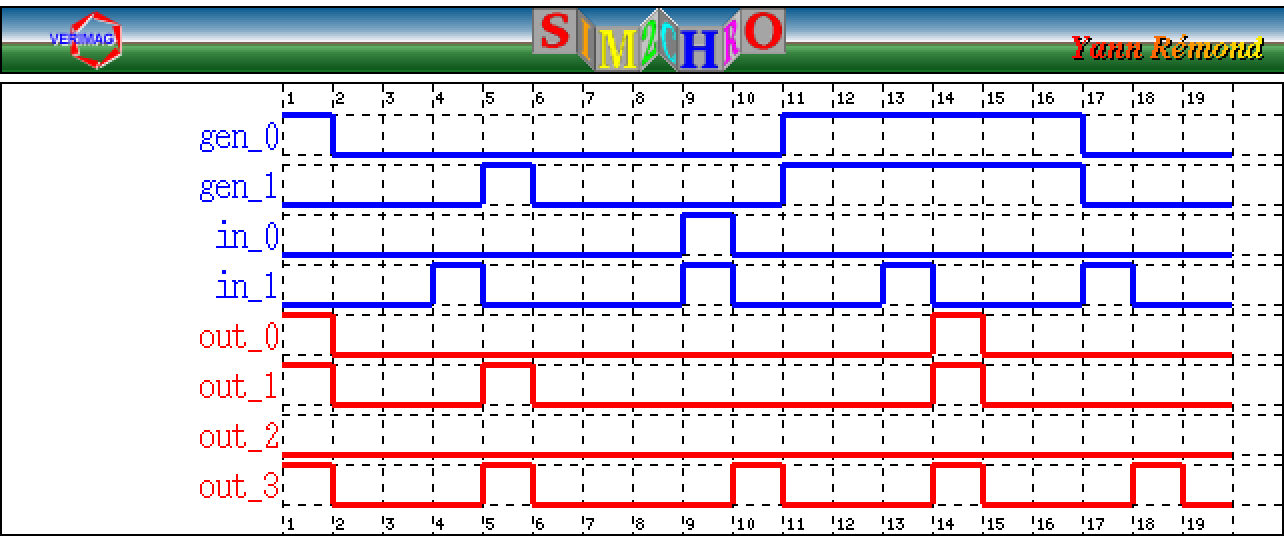
\includegraphics[width = 10cm]{cpu_diag.png}
		\caption{CPU}
	\end{figure}
	
\chapter{Arbitre}
	\begin{framed}
		\begin{verbatim}
		node arb(in: bool^3; valid: bool) returns (out: int);

--in: L1_1, L1_2, L1_3
--valid
--out: le cache choisit(resp. 1, 2, 3) et le mémoire(0)
--last: le dernier cache choisit sauf le mémoire
--commad: vaut true si le dernier out est un des caches sinon 
	vaut false

var
    last: int;
    command: bool;

let
    last = 0 -> if pre out <> 0 then pre out else pre last;
    command = false -> if out <> 0 then true
                else if out = 0 and valid then false
                else if out = 0 and not pre command 
                		then false
                else pre command
                ;

    out = 0 -> if pre command then 0
                else if last = 0 then
                    if in[0] then 1
                    else if in[1] then 2
                    else if in[2] then 3
                    else pre out
                else if pre last = 3 and in[0] then 1
                else if pre last = 1 and in[1] then 2
                else if pre last = 2 and in[2] then 3
                else if in[0] and not in[1] and not in[2] 
                		then 1
                else if in[1] and not in[2] and not in[0] 
                		then 2
                else if in[2] and not in[0] and not in[1] 
                		then 3
                else if in[0] and in[1] and not in[2] then 1
                else if in[1] and in[2] and not in[0] then 2
                else if in[2] and in[0] and not in[1] then 3
                else pre out
                ;

tel;
		\end{verbatim}
	\end{framed}
	
	L'arbitre prend en entrée 2 entrées $in$ de 3 bits et $valid$ de 1 bit. Si il y a plusieurs de requêtes simultanément, il va choisir le cache le plus prioritaire selon le numéro de cache et le dernier cache qui a utilisé le bus. Après un cycle, il rend le bus au mémoire, tant que le mémoire ne valide pas le bus( ne répond pas la requête du cache), le bus est toujours au mémoire. Si il y a des caches qui ne déactivent pas le signal de requête même si ils ont eu la réponse valide du mémoire, l'arbitre va rendre le bus au autre\footnote{Le cache dans ce programme n'a pas de comportement mauvais}.	
	
	\begin{figure}[!htbp]
		
		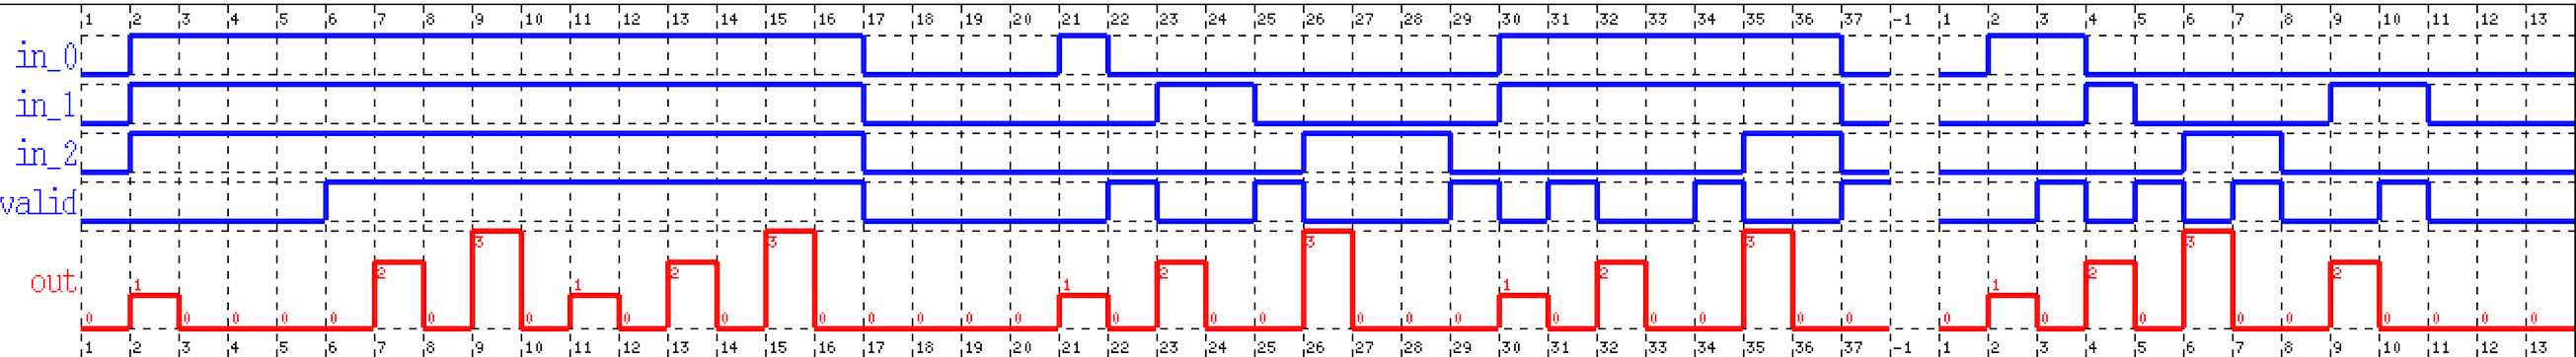
\includegraphics[width = 16cm]{arb_diag_1.png}
		\caption{Le cache ne rend pas le bus aux autres}
	\end{figure}
	\begin{figure}[!htbp]
		\centering
		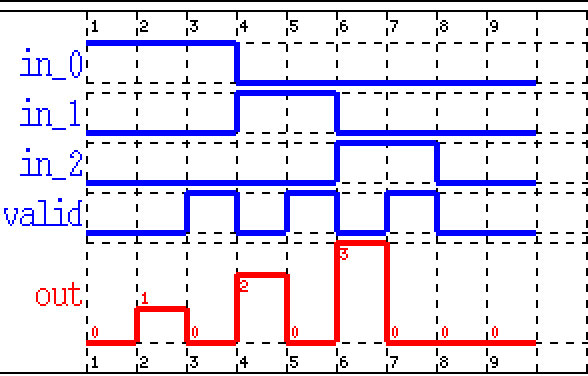
\includegraphics[width = 10cm]{arb_diag_2.png}
		\caption{Le comportement normal du cache}
	\end{figure}
	
\chapter{Mémoire}
	\begin{framed}
		\begin{verbatim}
		node mem(in: bool^4)returns (out: bool^4);

--in, out: typedata, adresse, data, valid
--reg0, reg1: 2 registres locals

var reg0, reg1: bool;

let
    reg0 = if in[3] and in[0] and not (in[1])
                then
                    in[2]
                else false -> pre reg0
                ;
    reg1 = if in[3] and in[0] and in[1]
                then
                    in[2]
                else false -> pre reg1
                ;

    out[0] = -- if false -> pre in[3] then
                    false -> pre in[0]
--                else false
            ;
    out[1] = --if false -> pre in[3] then
                    false -> pre in[1]
   --             else false
            ;
    out[2] = if false -> pre in[1] then
                    pre reg1
                else
                    false -> pre reg0
            ;
    out[3] = false -> pre in[3]
            ;

tel;

		\end{verbatim}
	\end{framed}
	
	Le mémoire regard les données entrantes, si elles sont valides, il répond en mettant la réponse dans sa boîte aux lettres sur le bus, il prend un cycle pour traiter un requête. Au début, les données sur le mémoire sont mise à 0.
	
	\begin{figure}[!htbp]
		
		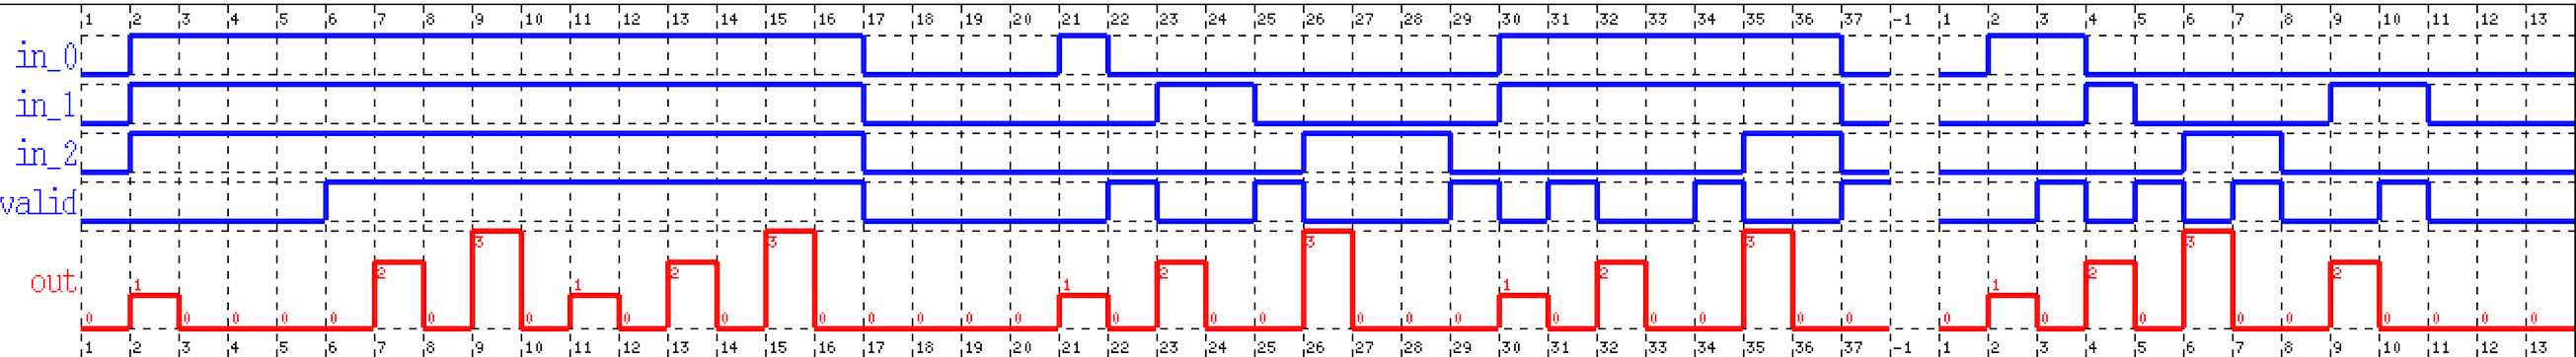
\includegraphics[width = 16cm]{arb_diag_1.png}
		\caption{Le cache ne rend pas le bus aux autres}
	\end{figure}
	
\chapter{Bus}
	\begin{framed}
		\begin{verbatim}
		node bus(in_1, in_2, in_3, in_mem: bool^4; arg_gnt: int) 
			returns (out: bool^4);

--in_1( resp. 2, 3, mem): l'entrée dans le bus mais les 
	données entrées sont toujours dans le bus, elles ne peuvent 
	sortir que si l'arbitre leurs donne la permission
--temp1( resp. 2, 3, 4): b_in_L1_1 et b_in_mem dans l'énoncé


var temp1, temp2, temp3, temp4: bool^3;

let
    temp1[0] = if false -> in_1[3] then in_1[0]
                    else false -> pre temp1[0];
    temp1[1] = if false -> in_1[3] then in_1[1]
                    else false -> pre temp1[1];
    temp1[2] = if false -> in_1[3] then in_1[2]
                    else false -> pre temp1[2];

    temp2[0] = if false -> in_2[3] then in_2[0]
                    else false -> pre temp2[0];
    temp2[1] = if false -> in_2[3] then in_2[1]
                    else false -> pre temp2[1];
    temp2[2] = if false -> in_2[3] then in_2[2]
                    else false -> pre temp2[2];

    temp3[0] = if false -> in_3[3] then in_3[0]
                    else false -> pre temp3[0];
    temp3[1] = if false -> in_3[3] then in_3[1]
                    else false -> pre temp3[1];
    temp3[2] = if false -> in_3[3] then in_3[2]
                    else false -> pre temp3[2];

    temp4[0] = if false -> in_mem[3] then in_mem[0]
                    else false -> pre temp4[0];
    temp4[1] = if false -> in_mem[3] then in_mem[1]
                    else false -> pre temp4[1];
    temp4[2] = if false -> in_mem[3] then in_mem[2]
                    else false -> pre temp4[2];

    out[0..2] = if arg_gnt = 3 then
                    temp3[0..2]
                else if arg_gnt = 1 then
                    temp1[0..2]
                else if arg_gnt = 2 then
                    temp2[0..2]
                else
                    temp4[0..2]
                ;
    out[3] = (0 -> pre arg_gnt <> 0 and arg_gnt = 0)
                or (0 -> pre arg_gnt = 0 and arg_gnt <> 0)
                ;

tel;

		\end{verbatim}
	\end{framed}
\chapter{Cache}
	\begin{framed}
		\begin{verbatim}
		node cache(in_arb: int; in_cpu: bool^4; in_bus: bool^4)
    returns (out_arb: bool; out_cpu: bool^2; out_bus: bool^4);

--in_arb: le numéro actuel de ce qui a la permission d'accès 
	au bus
--in_cpu: typedata, adresse, data, valid
--in_bus: typedata, adresse, data, valid

--out_arb: vaut 1 si le cache veut le bus sinon 0, le signal 
	maintient jusqu'à qu'il recoit la réponse du mémoire
--out_cpu: data, valid, valid vaut 1 si la réponse est valide 
	et l'acquittement du cache
--out_bus: typedata, adresse, data, valid

--data: le registre local dans le cache
--cpu_req: stock la requete de CPU précedente ou en traitement
--data_valid: vaut 1 si les données stockent dans le cache est 
	correspond avec la requête de CPU
--read, write: l'etat actuel du traitement
--write_valid: vaut 1 si les données sont valides sur le cache 
	donc il peut répondre tout de suite au CPU sinon vaut 0


var data: bool^2;
    cpu_req: bool^3;
    data_valid: bool;
    read, write: bool;
    write_valid: bool;

let

    cpu_req[0] = if in_cpu[3] then in_cpu[0] 
    					else false -> pre cpu_req[0]
                    ;
    cpu_req[1] = if in_cpu[3] then in_cpu[1] 
    					else false -> pre cpu_req[1]
                    ;
    cpu_req[2] = if in_cpu[3] then in_cpu[2] 
    					else false -> pre cpu_req[2]
                    ;

    out_bus[0] = cpu_req[0]
        ;
    out_bus[1] = cpu_req[1]
        ;
    out_bus[2] = cpu_req[2]
        ;
    out_bus[3] = cpu_req[0] or not (data_valid)
        ;

    data_valid = not( cpu_req[1] xor (false -> pre data[0]))
        ;

    data[0] = if not data_valid
                    and 0 -> pre in_arb = 2
                    and in_arb = 0
                    and in_bus[3] then
                        if (not in_bus[1] 
                        		and false -> pre data[0])
                            or (in_bus[1] 
                            	and not (false -> pre data[0]))
                        then in_bus[1]
                        else false -> pre data[0]
                else false -> pre data[0]
        ;
    data[1] = if not data_valid
                and 0 -> pre in_arb = 2
                and in_arb = 0
                and in_bus[3]
                then
                    in_bus[2]
                else if data_valid
                        and in_arb = 0
                        and in_bus[3]
                        and (data[0] and in_bus[1]
                        	or not (data[0]) 
                        	and not (in_bus[1])) then
                            in_bus[2]
                    else if data_valid and write then
                        in_cpu[2]
                    else false -> pre data[1]
        ;

    write_valid = if in_cpu[3] and in_cpu[0] then false
                    else if in_bus[0]
                            and in_bus[3]
                            and 0 -> pre in_arb = 2
                            and in_arb = 0
                        then true
                        else true -> pre write_valid
        ;

    out_arb = not data_valid
                or not write_valid
        ;

    read = if in_cpu[3] then
                if not in_cpu[0] then true
                else false
            else false -> pre read
        ;
    write = if in_cpu[3] then
                if in_cpu[0] then true
                else false
            else false -> pre write
        ;

    out_cpu[0] = if data_valid and read then data[1]
                    else false
        ;
    out_cpu[1] = if data_valid then true else false
        ;

tel;

		\end{verbatim}
	\end{framed}

\end{document}














